% Volume I: Mathematical Language and Finite-Dimensional Geometry
% Continuity note for Chapter 6.
% Previous dependencies: Chapter 3's vector geometry, bases, norms, inner products, angles, and orthogonal decomposition; Chapter 4's matrices as linear maps, rank, column space, null space, and change of basis; Chapter 5's projections, Gram matrices, QR coordinates, and least-squares approximation.
% New durable concepts: eigenvalues and eigenvectors as invariant directions; spectrum, characteristic polynomial, eigenspaces, and diagonalization; symmetric spectral theorem; quadratic forms, positive definiteness, semidefiniteness, and curvature; singular value decomposition; singular values and singular vectors; low-rank approximation; PCA as variance-preserving projection; scores, loadings, covariance eigenvectors, and reconstruction error.
% Forward hooks: Chapter 7 reuses SVD shapes, orthogonal factors, and matrix products in tensor operations and matrix calculus; Chapters 9-10 reuse quadratic forms as Hessian curvature and local optimization geometry; later dynamics chapters reuse eigenvalues for stability; probability and statistics chapters reuse covariance spectra, Gaussian ellipses, dimensionality reduction, neural population covariance, and representation geometry.
% Notation commitments: Square matrices use A in R^{n x n} for eigenvalue and quadratic-form sections; eigenpairs satisfy Av=lambda v with v nonzero; E_lambda=N(A-lambda I); Q is an orthogonal eigenvector matrix for symmetric matrices with A=Q Lambda Q^T; general rectangular maps use A in R^{m x n} with SVD A=U Sigma V^T; singular values sigma_i are nonnegative and ordered sigma_1 >= sigma_2 >= ...; centered data matrices use X in R^{N x p}, covariance C=(1/N)X^T X, principal directions w_i or columns of V, scores Z=XV_k, and reconstruction Xhat=XV_kV_k^T.
% Figure plan: four ImageGen raster figures are used and referenced: invariant eigen-directions for 6.1; quadratic-form contours and curvature for 6.2; SVD input-output axes for 6.3; PCA variance/projection geometry for 6.4.
\section{Chapter 6: Eigenvalues, SVD, Quadratic Forms, and PCA}
\label{ch:eigenvalues-svd-quadratic-forms-pca}

Chapters 4 and 5 taught us to read a matrix as a transformation and to use orthogonality to find best approximations. This chapter asks a more diagnostic question: does the transformation itself have preferred directions? Some directions pass through a square matrix without turning. Some directions make a symmetric quadratic form grow quickly. Some input directions are amplified most by a rectangular matrix. Some directions in a data cloud carry most of its variance.

The central problem is to find the coordinate systems in which a matrix or data set becomes geometrically simple. Eigenvectors reveal invariant directions of square maps. The spectral theorem turns symmetric matrices into orthogonal axes and scalar curvatures. The singular value decomposition gives paired input and output axes for any matrix. PCA uses the same spectral geometry to choose low-dimensional projections that preserve variance.

\paragraph{Chapter problem.}
How do we find the preferred directions of a transformation, an energy function, or a data cloud, and how do those directions support dynamics, curvature, compression, and representation analysis?

\paragraph{Section map.}
Section 6.1 defines eigenvalues and eigenvectors as invariant directions of square matrices. Section 6.2 specializes to symmetric matrices, where orthogonal eigenvectors make quadratic forms, covariance, and curvature transparent. Section 6.3 extends preferred-direction geometry to rectangular matrices through the singular value decomposition. Section 6.4 applies this geometry to PCA, where covariance eigenvectors define variance-preserving projection subspaces.

\subsection{6.1 Eigenvalues and eigenvectors}

\paragraph{Motivating question.}
For a square linear map \(A:\mathbb{R}^n\to\mathbb{R}^n\), which nonzero input directions keep the same direction after applying \(A\)?

\paragraph{Beginner setup.}
An \emph{eigenvector} is a nonzero vector whose direction is preserved by a square matrix. The matrix may stretch it, shrink it, reverse it, or collapse it to zero, but the output still lies on the same line through the origin. The scaling number is the \emph{eigenvalue}.

The smallest nontrivial example is a diagonal matrix:
\[
A=
\begin{bmatrix}
3&0\\
0&1/2
\end{bmatrix}.
\]
The horizontal vector \(e_1=(1,0)^\top\) satisfies
\[
Ae_1=3e_1,
\]
so \(e_1\) is an eigenvector with eigenvalue \(3\). The vertical vector \(e_2=(0,1)^\top\) satisfies
\[
Ae_2=\frac12 e_2,
\]
so \(e_2\) is an eigenvector with eigenvalue \(1/2\). But \(x=(1,1)^\top\) is not an eigenvector, because
\[
Ax=(3,1/2)^\top
\]
does not point in the same direction as \((1,1)^\top\).

Eigenvectors solve a reading problem. A generic matrix mixes coordinates, so it can be hard to predict repeated application, stability, or dominant variance directions. Eigenvectors identify directions where the matrix acts like scalar multiplication.

What to keep in mind: an eigenvector is a direction, not a unique arrow length. If \(v\) is an eigenvector, then any nonzero multiple \(cv\) is an eigenvector with the same eigenvalue. The zero vector is excluded because it has no direction and would satisfy \(A0=\lambda 0\) for every \(\lambda\).

\begin{figure}[htbp]
\centering
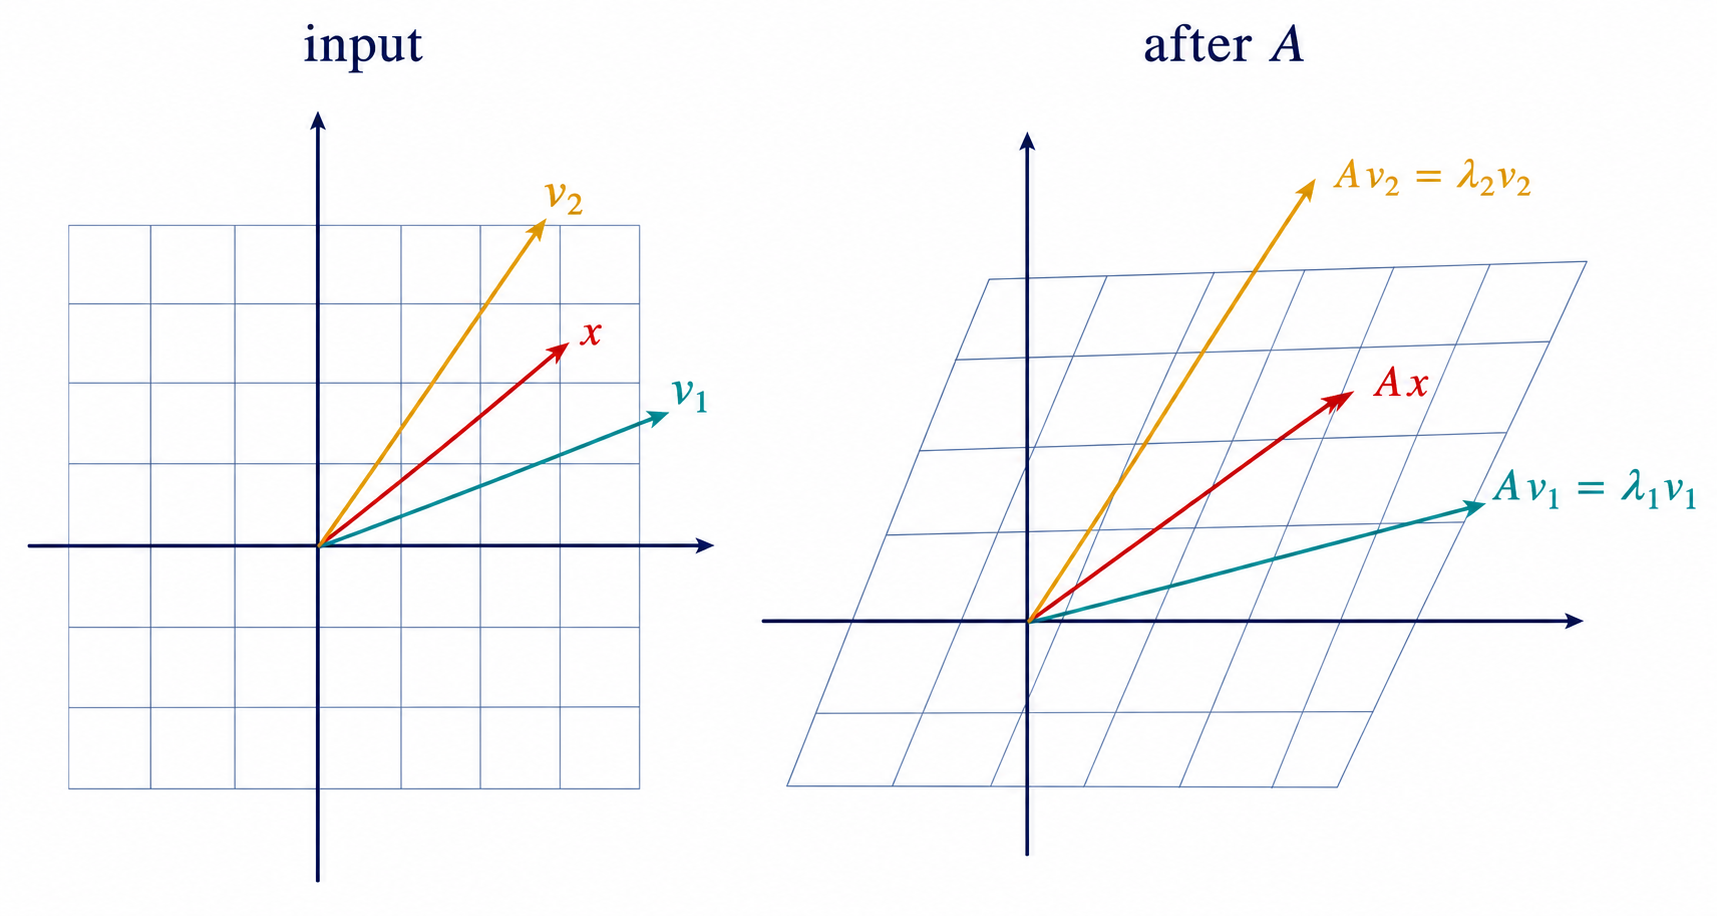
\includegraphics[width=0.95\linewidth]{imagegen-figures/ch06-eigen-invariant-directions.png}
\caption{Eigenvectors are invariant directions of a square linear map. The teal and gold directions remain on their original lines after applying \(A\), so \(Av_1=\lambda_1 v_1\) and \(Av_2=\lambda_2 v_2\). The red vector is not aligned with one invariant direction, so \(Ax\) generally turns.}
\label{fig:ch06-eigen-invariant-directions}
\end{figure}

\paragraph{Formal setup.}
Let \(A\in\mathbb{R}^{n\times n}\). A scalar \(\lambda\in\mathbb{R}\) is an \emph{eigenvalue} of \(A\) if there exists a nonzero vector \(v\in\mathbb{R}^n\) such that
\[
Av=\lambda v.
\]
The nonzero vector \(v\) is an \emph{eigenvector} associated with \(\lambda\). This is the central equation of the section. It only makes sense for square matrices because \(Av\) and \(v\) must live in the same vector space.

Rearranging gives
\[
(A-\lambda I)v=0.
\]
Thus eigenvectors for \(\lambda\) are nonzero vectors in the null space
\[
E_\lambda=N(A-\lambda I),
\]
called the \emph{eigenspace}. A nonzero null vector exists exactly when \(A-\lambda I\) is singular, so eigenvalues satisfy the \emph{characteristic equation}
\[
\det(A-\lambda I)=0.
\]
The set of eigenvalues is the \emph{spectrum} of \(A\).

\paragraph{Core intuition.}
Figure~\ref{fig:ch06-eigen-invariant-directions} shows the essential geometry. Most vectors are mixtures of several directions, and a matrix can change the relative amounts of those directions. A vector on an eigenline has no competing direction mixed into it, so the output remains on the same line.

Eigenvalues become especially informative when a map is applied repeatedly. If \(Av=\lambda v\), then
\[
A^2v=A(\lambda v)=\lambda Av=\lambda^2v,
\]
and, by repeating the same argument,
\[
A^kv=\lambda^k v.
\]
So \(|\lambda|<1\) means that component decays under repeated application, \(|\lambda|>1\) means it grows, \(\lambda<0\) means signs alternate, and \(\lambda=0\) means the direction is collapsed in one step.

Common misconceptions are worth removing early. First, an eigenvalue is not the length of \(Av\); it is the signed scaling relating \(Av\) to \(v\). Second, not every vector is an eigenvector. Third, not every real matrix has enough real eigenvectors to form a basis. A planar rotation by \(90^\circ\), for example, has no nonzero real vector whose direction is preserved. This chapter stays in real-vector geometry; complex eigenvalues and complex eigenvectors explain such rotations cleanly, but they are outside our present scope.

This section extends Chapter 4's matrix-as-map viewpoint and Chapter 5's interest in special orthogonal directions. It prepares linear dynamical systems, stability, covariance analysis, optimization curvature, and spectral graph methods.

\paragraph{Main theorem: diagonalization from an eigenbasis.}
Suppose \(A\in\mathbb{R}^{n\times n}\) has \(n\) linearly independent eigenvectors \(v_1,\dots,v_n\) with eigenvalues \(\lambda_1,\dots,\lambda_n\). Let
\[
V=
\begin{bmatrix}
v_1&v_2&\cdots&v_n
\end{bmatrix},
\qquad
\Lambda=
\begin{bmatrix}
\lambda_1&0&\cdots&0\\
0&\lambda_2&\cdots&0\\
\vdots&\vdots&\ddots&\vdots\\
0&0&\cdots&\lambda_n
\end{bmatrix}.
\]
Then \(V\) is invertible and
\[
A=V\Lambda V^{-1}.
\]
Consequently,
\[
A^k=V\Lambda^kV^{-1}.
\]

\emph{Proof sketch.} The equation \(Av_j=\lambda_jv_j\) says what \(A\) does to the \(j\)th column of \(V\). Putting all columns together gives
\[
AV=
\begin{bmatrix}
Av_1&Av_2&\cdots&Av_n
\end{bmatrix}
=
\begin{bmatrix}
\lambda_1v_1&\lambda_2v_2&\cdots&\lambda_nv_n
\end{bmatrix}
=V\Lambda.
\]
Because the eigenvectors are linearly independent, \(V\) is invertible. Multiplying \(AV=V\Lambda\) on the right by \(V^{-1}\) gives \(A=V\Lambda V^{-1}\). Repeated powers follow because the middle factors cancel:
\[
A^2=(V\Lambda V^{-1})(V\Lambda V^{-1})=V\Lambda^2V^{-1},
\]
and the same cancellation gives \(A^k=V\Lambda^kV^{-1}\).

\paragraph{Worked examples.}
\emph{Small numerical example.} Let
\[
A=
\begin{bmatrix}
2&1\\
0&3
\end{bmatrix}.
\]
The characteristic polynomial is
\[
\det(A-\lambda I)
=
\det
\begin{bmatrix}
2-\lambda&1\\
0&3-\lambda
\end{bmatrix}
=(2-\lambda)(3-\lambda).
\]
So the eigenvalues are \(2\) and \(3\).

For \(\lambda=2\),
\[
A-2I=
\begin{bmatrix}
0&1\\
0&1
\end{bmatrix},
\]
so \(y=0\) and \(v_1=(1,0)^\top\) is an eigenvector. For \(\lambda=3\),
\[
A-3I=
\begin{bmatrix}
-1&1\\
0&0
\end{bmatrix},
\]
so \(y=x\) and \(v_2=(1,1)^\top\) is an eigenvector. The matrix stretches the horizontal direction by \(2\) and the diagonal direction \((1,1)\) by \(3\).

\emph{ML/neuroscience example.} A linear recurrent model has hidden state
\[
h_{t+1}=Wh_t.
\]
If \(Wv=\lambda v\), then activity initialized along \(v\) evolves as \(h_t=\lambda^t v\). A mode with \(|\lambda|=0.8\) decays, a mode with \(|\lambda|=1.05\) grows, and a mode with \(\lambda=-0.9\) alternates sign while decaying. In neural population models, eigenvectors of a fitted recurrent matrix identify activity patterns, and eigenvalues summarize whether those patterns are stable, persistent, oscillatory, or unstable in the linear approximation.

\paragraph{ML/DL/neuroscience connections.}
In recurrent neural networks, eigenvalues of the recurrent weight matrix control gradient and activity amplification in linearized regimes. In optimization, eigenvectors of a Hessian mark curvature directions and eigenvalues say whether the loss rises steeply or shallowly. In neuroscience, eigenvectors of linear dynamics or covariance matrices describe population modes: patterns of co-activation across neurons. The objects are concrete: the matrix is a transition, covariance, Hessian, or connectivity estimate; the eigenvectors are activity or parameter directions; the eigenvalues are gains, variances, or curvatures.

\paragraph{Exercises.}
\begin{enumerate}[label=\textbf{6.1.\arabic*.}, leftmargin=*]
\item \textbf{Mechanical.} For
\[
A=\begin{bmatrix}4&1\\0&2\end{bmatrix},
\]
compute the eigenvalues and one eigenvector for each eigenvalue.
\item \textbf{Proof or derivation.} Suppose \(Av=\lambda v\) and \(Aw=\mu w\), where \(\lambda\neq\mu\). Prove that \(v\) and \(w\) are linearly independent.
\item \textbf{Numerical/computational.} Write pseudocode that forms the characteristic polynomial of a \(2\times 2\) matrix, solves for its eigenvalues, and then finds a null vector of \(A-\lambda I\) for each eigenvalue.
\item \textbf{Interpretation.} In the recurrent system \(h_{t+1}=Wh_t\), what happens to a component of \(h_0\) along an eigenvector with eigenvalue \(0.2\), with eigenvalue \(1.3\), and with eigenvalue \(-0.7\)?
\item \textbf{Debug the misconception.} A student says, ``The eigenvector is the vector that gets the largest output.'' Explain why eigenvectors are about preserved direction, not necessarily largest amplification.
\end{enumerate}

\subsection{6.2 Symmetric matrices and quadratic forms}

\paragraph{Motivating question.}
How does a symmetric matrix assign an energy or curvature value to each direction in space?

\paragraph{Beginner setup.}
A \emph{symmetric matrix} satisfies \(A^\top=A\). Symmetry means that the interaction from coordinate \(i\) to coordinate \(j\) matches the interaction from coordinate \(j\) to coordinate \(i\). A \emph{quadratic form} built from \(A\) is the scalar-valued function
\[
q(x)=x^\top A x.
\]
It takes a vector \(x\in\mathbb{R}^n\) and returns a number.

The smallest clear example is
\[
A=
\begin{bmatrix}
4&0\\
0&1
\end{bmatrix}.
\]
Then
\[
q(x)=x^\top A x
=4x_1^2+x_2^2.
\]
The level set \(q(x)=1\) is an ellipse. Moving in the \(x_1\) direction makes \(q\) grow quickly, because the coefficient \(4\) is large. Moving in the \(x_2\) direction makes it grow more slowly.

Quadratic forms solve the problem of measuring direction-dependent energy. They appear as squared distances, covariance ellipses, loss curvature, regularizers, Gaussian log densities, and physical energies. Symmetric matrices are the natural matrices for quadratic forms because the skew-symmetric part of a matrix contributes nothing to \(x^\top A x\).

What to keep in mind: \(A\) is still a linear map, but \(x^\top A x\) is not a linear map. It is a scalar energy-like quantity whose value depends on both the direction and length of \(x\).

\begin{figure}[htbp]
\centering
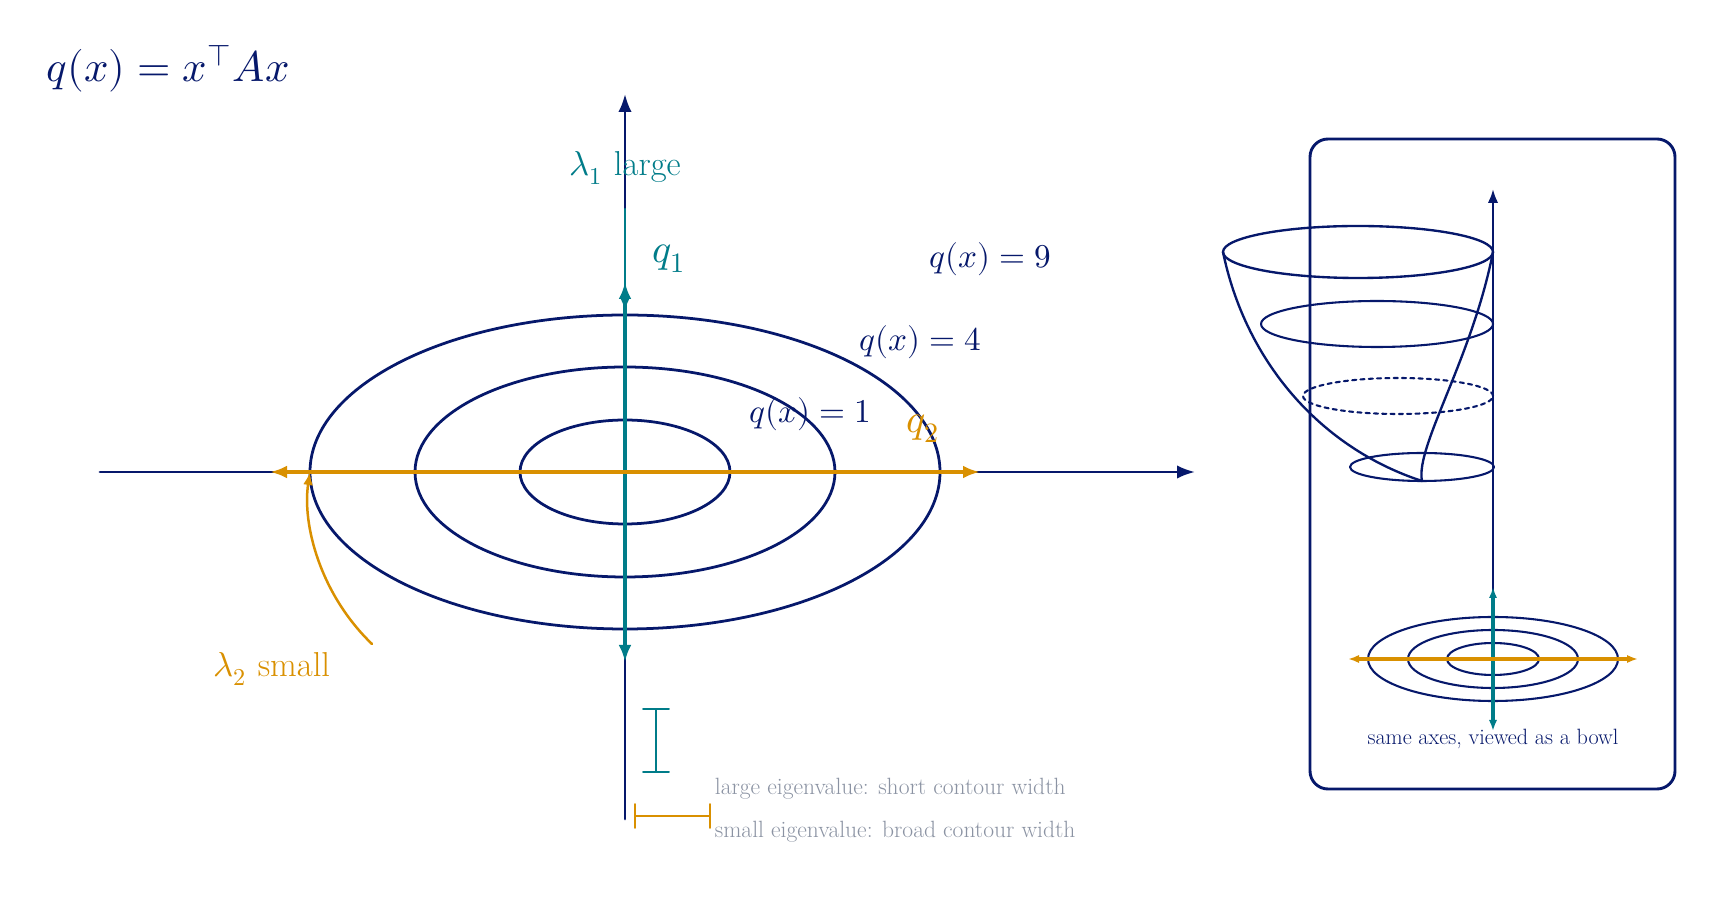
\includegraphics[width=0.95\linewidth]{imagegen-figures/ch06-quadratic-forms-contours.png}
\caption{A symmetric positive definite matrix defines elliptical level sets for \(q(x)=x^\top A x\). Orthogonal eigenvectors give the principal axes. Large eigenvalues produce tight curvature and narrow contour widths; small positive eigenvalues produce broad, shallow directions.}
\label{fig:ch06-quadratic-forms-contours}
\end{figure}

\paragraph{Formal setup.}
Let \(A\in\mathbb{R}^{n\times n}\) be symmetric. The associated quadratic form is
\[
q:\mathbb{R}^n\to\mathbb{R},
\qquad
q(x)=x^\top A x.
\]
The matrix \(A\) is \emph{positive definite} if
\[
x^\top A x>0
\qquad\text{for every }x\neq 0,
\]
and \emph{positive semidefinite} if
\[
x^\top A x\geq 0
\qquad\text{for every }x.
\]
If the quadratic form takes both positive and negative values, \(A\) is \emph{indefinite}.

The central coordinate simplification comes from the spectral theorem. A real symmetric matrix has an orthonormal eigenbasis:
\[
A=Q\Lambda Q^\top,
\qquad
Q^\top Q=I.
\]
If \(z=Q^\top x\) are the coordinates of \(x\) in the eigenvector basis, then
\[
q(x)=x^\top Q\Lambda Q^\top x
=z^\top\Lambda z
=\sum_{i=1}^n \lambda_i z_i^2.
\]
This equation says that in the right orthonormal coordinates, a symmetric quadratic form has no cross terms.

\paragraph{Core intuition.}
Figure~\ref{fig:ch06-quadratic-forms-contours} shows the picture in two dimensions. Level curves of a positive definite quadratic form are ellipses centered at the origin. The eigenvectors are the ellipse axes. Eigenvalues determine how fast the energy grows along each axis. A large eigenvalue means \(q\) becomes large after a short move, so the ellipse is narrow in that direction. A small positive eigenvalue means the form is shallow, so the ellipse stretches farther.

This is the same idea that later appears in optimization. Near a minimum, a smooth loss is often approximated by a quadratic expression. The Hessian matrix plays the role of \(A\): large positive eigenvalues are steep directions, small positive eigenvalues are flat directions, negative eigenvalues indicate a direction where the point is not a minimum, and zero eigenvalues indicate locally flat directions.

Common misconceptions come from forgetting the symmetry. First, not every square matrix has orthogonal eigenvectors. The orthogonal diagonalization \(A=Q\Lambda Q^\top\) is a special strength of real symmetric matrices. Second, positive entries do not guarantee positive definiteness; the eigenvalues determine definiteness. Third, a covariance matrix is positive semidefinite, not necessarily positive definite, because some directions may have zero variance.

\paragraph{Main theorem: spectral reading of quadratic forms.}
Let \(A\in\mathbb{R}^{n\times n}\) be symmetric with spectral decomposition \(A=Q\Lambda Q^\top\). Then
\[
x^\top A x=\sum_{i=1}^n \lambda_i z_i^2,
\qquad
z=Q^\top x.
\]
Therefore:
\[
A\text{ is positive definite}\Longleftrightarrow \lambda_i>0\text{ for all }i,
\]
\[
A\text{ is positive semidefinite}\Longleftrightarrow \lambda_i\geq 0\text{ for all }i.
\]

\emph{Proof sketch.} Since \(Q\) is orthogonal, changing coordinates from \(x\) to \(z=Q^\top x\) preserves lengths and angles. Substitute \(A=Q\Lambda Q^\top\):
\[
x^\top A x
=x^\top Q\Lambda Q^\top x.
\]
The expression \(x^\top Q\) equals \((Q^\top x)^\top=z^\top\), so
\[
x^\top A x=z^\top\Lambda z.
\]
Because \(\Lambda\) is diagonal, this is
\[
\lambda_1z_1^2+\cdots+\lambda_nz_n^2.
\]
If every \(\lambda_i>0\), every nonzero \(z\) makes the sum positive. If one \(\lambda_j<0\), choosing \(z=e_j\) makes the form negative. If one \(\lambda_j=0\) and the rest are nonnegative, the form is never negative but is zero along that eigenvector. This proves the definiteness criteria.

\paragraph{Worked examples.}
\emph{Small numerical example.} Let
\[
A=
\begin{bmatrix}
2&1\\
1&2
\end{bmatrix}.
\]
The vectors
\[
q_1=\frac{1}{\sqrt2}\begin{bmatrix}1\\1\end{bmatrix},
\qquad
q_2=\frac{1}{\sqrt2}\begin{bmatrix}1\\-1\end{bmatrix}
\]
are orthonormal eigenvectors. A direct multiplication gives
\[
Aq_1=3q_1,
\qquad
Aq_2=q_2.
\]
Thus
\[
Q=
\begin{bmatrix}
1/\sqrt2&1/\sqrt2\\
1/\sqrt2&-1/\sqrt2
\end{bmatrix},
\qquad
\Lambda=
\begin{bmatrix}
3&0\\
0&1
\end{bmatrix},
\]
and \(A=Q\Lambda Q^\top\). In eigen-coordinates \(z=Q^\top x\),
\[
x^\top A x=3z_1^2+z_2^2.
\]
The form is positive definite because both eigenvalues are positive. It is steeper along \(q_1\) than along \(q_2\).

\emph{ML/neuroscience example.} Let \(X\in\mathbb{R}^{N\times p}\) be centered neural population data, with rows as trials and columns as neurons. The covariance matrix
\[
C=\frac{1}{N}X^\top X
\]
is symmetric positive semidefinite. For any unit vector \(w\in\mathbb{R}^p\),
\[
w^\top Cw
=\frac{1}{N}\|Xw\|^2
\]
is the variance of the population activity after projecting each trial onto direction \(w\). Eigenvectors of \(C\) are orthogonal population patterns. Eigenvalues are variances along those patterns.

\paragraph{ML/DL/neuroscience connections.}
In machine learning, quadratic forms appear in regularization terms such as \(w^\top \Gamma w\), in Mahalanobis distances \((x-\mu)^\top\Sigma^{-1}(x-\mu)\), and in second-order approximations to loss functions. In deep learning, Hessian eigenvalues diagnose sharp and flat parameter directions. In neuroscience, covariance matrices and noise covariance matrices are symmetric positive semidefinite; their eigenvectors are neural population modes and their eigenvalues quantify trial-to-trial variability along those modes.

\paragraph{Exercises.}
\begin{enumerate}[label=\textbf{6.2.\arabic*.}, leftmargin=*]
\item \textbf{Mechanical.} For
\[
A=\begin{bmatrix}5&0\\0&2\end{bmatrix},
\]
write \(q(x)=x^\top A x\), sketch the relative shape of \(q(x)=1\), and state whether \(A\) is positive definite.
\item \textbf{Proof or derivation.} Let \(A\) be any square matrix and write \(A=S+K\), where \(S=(A+A^\top)/2\) and \(K=(A-A^\top)/2\). Prove that \(x^\top Kx=0\) for every \(x\), so \(x^\top A x=x^\top Sx\).
\item \textbf{Numerical/computational.} Given a symmetric matrix \(A\), write pseudocode that computes eigenvalues, checks whether all are positive, nonnegative, or mixed in sign, and returns positive definite, positive semidefinite, or indefinite.
\item \textbf{Interpretation.} A loss Hessian has eigenvalues \(100\), \(2\), and \(0.01\). What do these numbers say about the local shape of the loss in the corresponding eigenvector directions?
\item \textbf{Debug the misconception.} A student says, ``This matrix has only positive entries, so its quadratic form must be positive definite.'' Give a counterexample or explain why eigenvalues, not entry signs, decide definiteness.
\end{enumerate}

\subsection{6.3 Singular value decomposition}

\paragraph{Motivating question.}
For a possibly rectangular matrix \(A:\mathbb{R}^n\to\mathbb{R}^m\), can we find orthonormal input directions, orthonormal output directions, and nonnegative gains connecting them?

\paragraph{Beginner setup.}
Eigenvectors require a square map from a space back to itself. Many important matrices are rectangular: a data matrix maps feature weights to predictions, a neural layer maps one activation dimension to another, and a measurement matrix maps latent variables to sensors. The \emph{singular value decomposition}, or SVD, gives preferred directions for any matrix.

The smallest geometric example is
\[
A=
\begin{bmatrix}
3&0\\
0&1
\end{bmatrix}.
\]
It maps the unit circle to an ellipse. The horizontal input direction is stretched by \(3\), the vertical input direction is stretched by \(1\), and the output axes are the same as the input axes. A general matrix first chooses orthonormal input axes, then stretches by nonnegative amounts, then rotates or reflects into orthonormal output axes.

SVD solves several problems at once. It measures which input directions are amplified or suppressed, reveals rank and null space, gives stable coordinates for least squares, and provides the best low-rank approximation to a matrix.

What to keep in mind: singular values are always nonnegative and always exist for real matrices. They are not the same as eigenvalues in general. Eigenvectors describe directions preserved by a square map; singular vectors describe paired input and output directions for any map.

\begin{figure}[htbp]
\centering
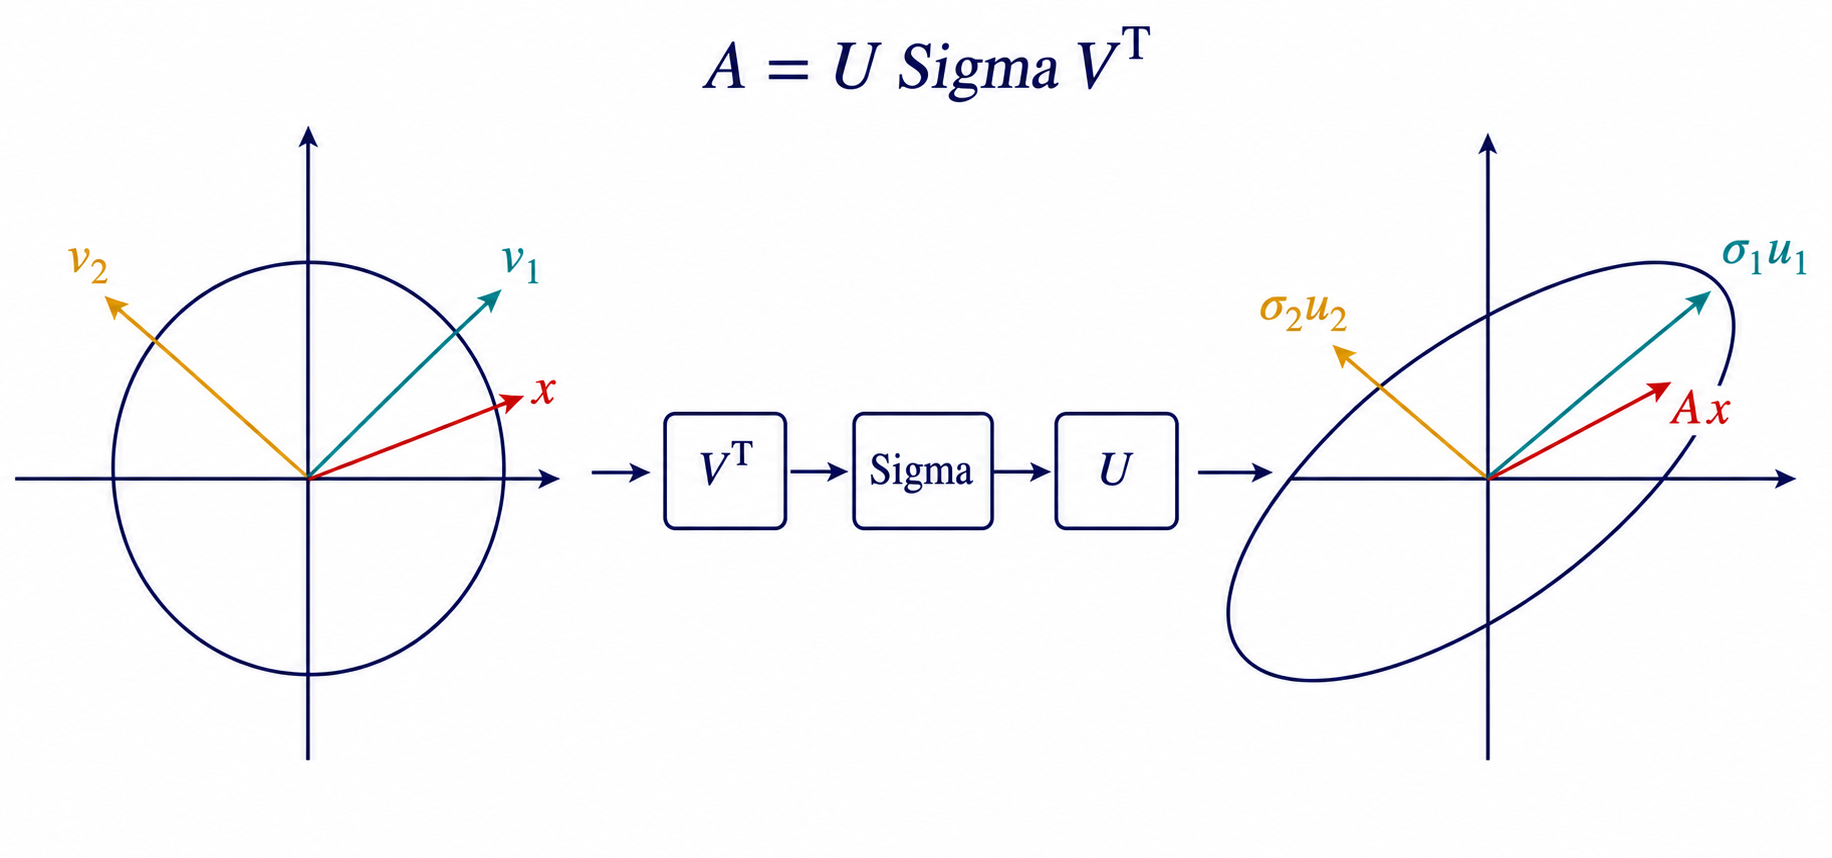
\includegraphics[width=0.95\linewidth]{imagegen-figures/ch06-svd-input-output-axes.png}
\caption{SVD decomposes a matrix into input axes, nonnegative stretches, and output axes. The right singular vectors \(v_i\) are orthonormal input directions. The left singular vectors \(u_i\) are orthonormal output directions. The singular values \(\sigma_i\) are the gains, so \(Av_i=\sigma_i u_i\).}
\label{fig:ch06-svd-input-output-axes}
\end{figure}

\paragraph{Formal setup.}
Let \(A\in\mathbb{R}^{m\times n}\). An SVD of \(A\) is a factorization
\[
A=U\Sigma V^\top,
\]
where \(U\in\mathbb{R}^{m\times m}\) is orthogonal, \(V\in\mathbb{R}^{n\times n}\) is orthogonal, and \(\Sigma\in\mathbb{R}^{m\times n}\) has nonnegative diagonal entries
\[
\sigma_1\geq\sigma_2\geq\cdots\geq 0.
\]
The columns \(v_i\) of \(V\) are \emph{right singular vectors}. The columns \(u_i\) of \(U\) are \emph{left singular vectors}. The nonzero singular values satisfy
\[
Av_i=\sigma_i u_i.
\]

If \(A\) has rank \(r\), its compact SVD is
\[
A=\sum_{i=1}^r \sigma_i u_i v_i^\top.
\]
The singular values are tied to symmetric eigenvalue problems:
\[
A^\top A=V(\Sigma^\top\Sigma)V^\top,
\qquad
AA^\top=U(\Sigma\Sigma^\top)U^\top.
\]
Thus \(\sigma_i^2\) are eigenvalues of \(A^\top A\) and \(AA^\top\).

\paragraph{Core intuition.}
Figure~\ref{fig:ch06-svd-input-output-axes} is the SVD picture. The unit circle in input space maps to an ellipse in output space. The directions \(v_i\) are the input directions that land exactly on the ellipse axes. The directions \(u_i\) are those output axes. The singular values \(\sigma_i\) are the semi-axis lengths.

The factorization \(A=U\Sigma V^\top\) can be read from right to left. First \(V^\top\) expresses the input in the right singular-vector coordinates. Then \(\Sigma\) scales each coordinate by a nonnegative singular value and may change the dimension. Finally \(U\) places the result in output coordinates.

Common misconceptions: First, SVD is not only for square matrices. It is most useful precisely because it works for rectangular matrices. Second, a zero singular value marks an input direction that the matrix sends to zero; it is a null-space direction. Third, a large singular value means large amplification of a particular input direction, not necessarily large entries in the matrix. Fourth, the signs of singular vectors are arbitrary: replacing both \(u_i\) and \(v_i\) by their negatives leaves \(\sigma_i u_i v_i^\top\) unchanged.

This section connects backward to Gram matrices from Chapter 5 because \(A^\top A\) compares columns by inner products. It connects forward to tensor decompositions, stable least squares, neural network weight analysis, randomized linear algebra, and representation compression.

\paragraph{Main theorem: SVD and best low-rank approximation.}
Every matrix \(A\in\mathbb{R}^{m\times n}\) has an SVD
\[
A=\sum_{i=1}^r\sigma_i u_i v_i^\top,
\qquad
\sigma_1\geq\cdots\geq\sigma_r>0.
\]
For \(k<r\), the truncated SVD
\[
A_k=\sum_{i=1}^k\sigma_i u_i v_i^\top
\]
is a best rank-\(k\) approximation to \(A\) in Frobenius norm:
\[
A_k\in\arg\min_{\operatorname{rank}(B)\leq k}\|A-B\|_F.
\]
The squared error is
\[
\|A-A_k\|_F^2=\sum_{i=k+1}^r\sigma_i^2.
\]
If there is a tie at the cutoff, such as \(\sigma_k=\sigma_{k+1}\), the best rank-\(k\) approximation need not be unique. Any choice that keeps a \(k\)-dimensional part of the tied singular subspace has the same optimal Frobenius error.

\emph{Proof sketch.} The full proof of existence uses the spectral theorem on \(A^\top A\). Since \(A^\top A\) is symmetric positive semidefinite, it has orthonormal eigenvectors \(v_i\) and nonnegative eigenvalues \(\sigma_i^2\). For each positive \(\sigma_i\), define
\[
u_i=\frac{Av_i}{\sigma_i}.
\]
One checks that the \(u_i\) are orthonormal and that \(Av_i=\sigma_i u_i\). Completing these to orthonormal bases gives \(U\) and \(V\), hence \(A=U\Sigma V^\top\).

For approximation, the singular-vector coordinates separate the matrix into orthogonal rank-one pieces \(\sigma_i u_i v_i^\top\). Their squared Frobenius norms are \(\sigma_i^2\), and different pieces are orthogonal under the matrix inner product. Keeping the \(k\) largest pieces preserves the most squared norm available to any rank-\(k\) approximation, so the discarded error is the sum of the remaining \(\sigma_i^2\). This is the Eckart-Young theorem.

\paragraph{Worked examples.}
\emph{Small numerical example.} For
\[
A=
\begin{bmatrix}
3&0\\
0&1
\end{bmatrix},
\]
we can take \(U=I\), \(V=I\), and
\[
\Sigma=
\begin{bmatrix}
3&0\\
0&1
\end{bmatrix}.
\]
The singular values are \(3\) and \(1\). The best rank-one approximation is
\[
A_1=
\begin{bmatrix}
3&0\\
0&0
\end{bmatrix},
\]
and the Frobenius error is
\[
\|A-A_1\|_F=1.
\]
Geometrically, the rank-one approximation keeps the long horizontal ellipse axis and discards the shorter vertical axis.

\emph{ML/neuroscience example.} Suppose \(W\in\mathbb{R}^{m\times n}\) is the weight matrix of a linear layer mapping an \(n\)-dimensional representation to an \(m\)-dimensional representation. The right singular vector \(v_1\) is the input activity pattern most amplified by the layer, and \(u_1\) is the corresponding output pattern. If most singular values after the first \(k\) are small, then
\[
W_k=\sum_{i=1}^k\sigma_i u_i v_i^\top
\]
is a low-rank compressed layer that keeps the dominant input-output relationships. In neuroscience, the same idea applies to a stimulus-to-response matrix: singular vectors pair stimulus features with neural population response patterns.

\paragraph{ML/DL/neuroscience connections.}
SVD is a diagnostic for linear layers, embeddings, and fitted encoding models. The matrix may be a weight matrix, a data matrix, a Jacobian, or a stimulus-response map. Right singular vectors are input patterns; left singular vectors are output patterns; singular values are gains. Low-rank truncation becomes compression, denoising, and dimensionality reduction. In recurrent and deep networks, the largest singular value controls worst-case one-step amplification even when eigenvalues alone do not describe transient growth.

\paragraph{Exercises.}
\begin{enumerate}[label=\textbf{6.3.\arabic*.}, leftmargin=*]
\item \textbf{Mechanical.} Find an SVD of
\[
A=\begin{bmatrix}2&0\\0&1\end{bmatrix}.
\]
Identify \(u_i\), \(v_i\), and \(\sigma_i\).
\item \textbf{Proof or derivation.} Starting from \(A=U\Sigma V^\top\), derive \(A^\top A=V(\Sigma^\top\Sigma)V^\top\). Explain why the eigenvalues of \(A^\top A\) are squared singular values.
\item \textbf{Numerical/computational.} Write pseudocode that takes a data matrix \(A\), computes its SVD, constructs \(A_k\), and reports the relative Frobenius reconstruction error \(\|A-A_k\|_F/\|A\|_F\).
\item \textbf{Interpretation.} A neural network layer has singular values \(9, 3, 0.2, 0.01\). What does this suggest about amplification, effective dimension, and possible low-rank approximation?
\item \textbf{Debug the misconception.} A student says, ``SVD is just eigenvectors for non-square matrices.'' Explain what is right in that intuition and what is missing.
\end{enumerate}

\subsection{6.4 Principal component analysis}

\paragraph{Motivating question.}
Which lower-dimensional subspace preserves as much variance as possible in centered data?

\paragraph{Beginner setup.}
Principal component analysis, or PCA, is projection geometry applied to data. Start with a data matrix
\[
X\in\mathbb{R}^{N\times p},
\]
where each row is one observation and each column is one measured feature. PCA assumes the columns have been centered, so each feature has mean zero. The sample covariance matrix is
\[
C=\frac{1}{N}X^\top X.
\]

A unit vector \(w\in\mathbb{R}^p\) defines a one-dimensional projection direction. The projected scores are \(Xw\in\mathbb{R}^N\). Their variance is
\[
\frac{1}{N}\|Xw\|^2
=w^\top Cw.
\]
PCA chooses the first principal component \(w_1\) to maximize this variance subject to \(\|w_1\|=1\). Later components maximize remaining variance while staying orthogonal to earlier components.

The smallest clear example is a centered two-dimensional data cloud that is longer in one direction than another. PCA finds the long direction first. Projecting onto that direction gives a one-dimensional summary; projecting back into the original feature space gives a reconstruction; the difference is reconstruction error.

What to keep in mind: PCA is unsupervised. It does not know labels or task goals. It finds high-variance directions, which may or may not be the directions most useful for prediction or interpretation. Centering is essential, and the sign of each principal component is arbitrary.

\begin{figure}[htbp]
\centering
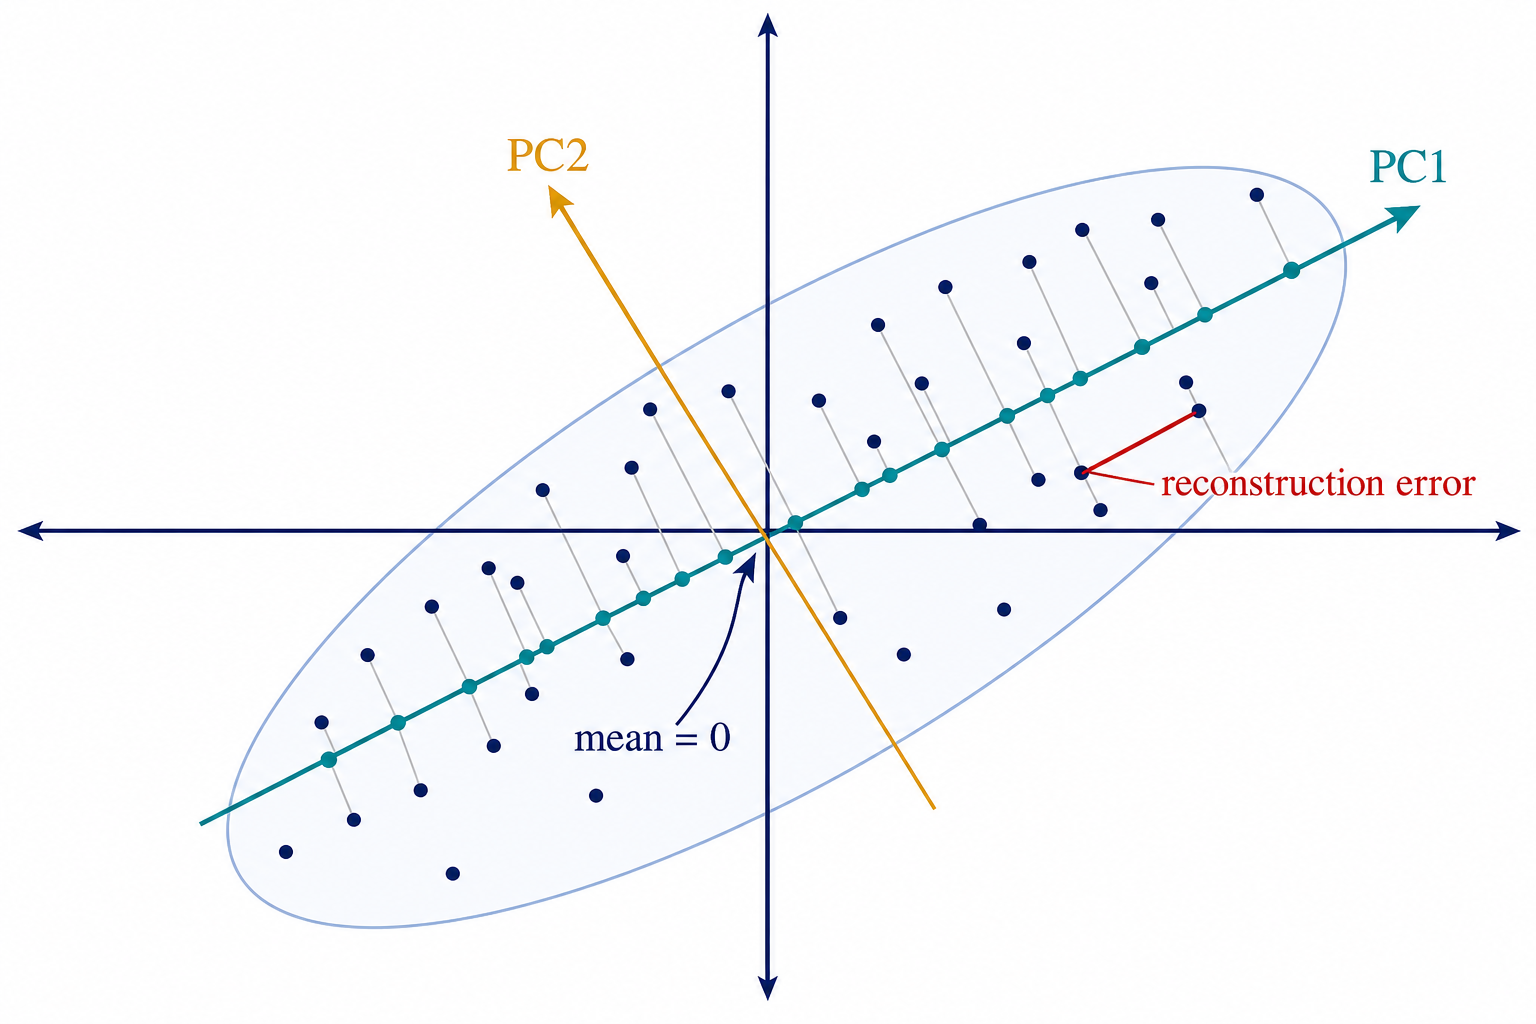
\includegraphics[width=0.95\linewidth]{imagegen-figures/ch06-pca-variance-geometry.png}
\caption{PCA chooses orthogonal directions in centered data. The first principal component follows the largest variance direction of the cloud. Projection onto PC1 gives a one-dimensional approximation; the discarded perpendicular pieces are reconstruction errors.}
\label{fig:ch06-pca-variance-geometry}
\end{figure}

\paragraph{Formal setup.}
Let \(X\in\mathbb{R}^{N\times p}\) be centered by columns:
\[
\sum_{i=1}^N X_{ij}=0
\qquad
\text{for each feature }j.
\]
Define
\[
C=\frac{1}{N}X^\top X\in\mathbb{R}^{p\times p}.
\]
The one-dimensional PCA problem is
\[
w_1=\arg\max_{\|w\|=1} w^\top Cw.
\]
For \(k\) components, let
\[
V_k=
\begin{bmatrix}
w_1&w_2&\cdots&w_k
\end{bmatrix}
\in\mathbb{R}^{p\times k},
\qquad
V_k^\top V_k=I_k.
\]
The \emph{scores} are
\[
Z=XV_k\in\mathbb{R}^{N\times k},
\]
and the rank-\(k\) reconstruction in the original feature space is
\[
\widehat X=ZV_k^\top=XV_kV_k^\top.
\]
Thus PCA is also a projection: each centered row vector is projected onto the subspace spanned by the first \(k\) principal directions.

If
\[
X=U\Sigma V^\top
\]
is an SVD, then
\[
C=\frac{1}{N}X^\top X
=V\left(\frac{1}{N}\Sigma^\top\Sigma\right)V^\top.
\]
So principal directions are right singular vectors of \(X\), and covariance eigenvalues are \(\sigma_i^2/N\).

\paragraph{Core intuition.}
Figure~\ref{fig:ch06-pca-variance-geometry} shows the same projection story as Chapter 5, but now the subspace is chosen from the data rather than specified in advance. A one-dimensional projection is good if the projected points stay spread out and the perpendicular reconstruction errors stay small. The first principal component is the unit direction that maximizes projected variance. The second principal component is the best remaining orthogonal direction, and so on.

The covariance matrix is the bridge between data and geometry. For a unit direction \(w\), the scalar \(w^\top Cw\) is the variance seen after projecting all rows of \(X\) onto \(w\). Section 6.2 taught us that the largest value of a symmetric quadratic form on the unit sphere occurs along the eigenvector with largest eigenvalue. PCA applies that result to \(C\).

Common misconceptions: First, PCA components are feature-space directions, not clusters of data points. Second, the first component is not always the most scientifically meaningful variable; it is the highest-variance linear direction. Third, PCA requires centering unless the goal is explicitly to analyze variation around the origin. Fourth, PCA loadings and scores are different objects: loadings live in feature space, while scores are coordinates of observations in the principal-component basis.

\paragraph{Main theorem: PCA variance and reconstruction.}
Let \(C=(1/N)X^\top X\) be the covariance matrix of centered data, with eigenvalues
\[
\lambda_1\geq\lambda_2\geq\cdots\geq\lambda_p\geq 0
\]
and orthonormal eigenvectors \(w_1,\dots,w_p\). Then \(w_1\) solves
\[
\max_{\|w\|=1}w^\top Cw.
\]
More generally, the subspace spanned by \(w_1,\dots,w_k\) maximizes total projected variance among all \(k\)-dimensional orthonormal subspaces:
\[
\max_{V^\top V=I_k}\operatorname{tr}(V^\top C V)
=\lambda_1+\cdots+\lambda_k.
\]
The same subspace minimizes squared reconstruction error:
\[
\min_{V^\top V=I_k}\|X-XVV^\top\|_F^2.
\]
When eigenvalues tie, PCA directions inside the tied eigenspace are not unique. If \(\lambda_k=\lambda_{k+1}\), there can be several equally good \(k\)-dimensional PCA subspaces with the same projected variance and reconstruction error.

\emph{Proof sketch.} Write \(C=Q\Lambda Q^\top\), and express any unit vector as \(w=Qz\), where \(\|z\|=1\). Then
\[
w^\top Cw=z^\top\Lambda z=\sum_{i=1}^p\lambda_i z_i^2.
\]
The numbers \(z_i^2\) are nonnegative and sum to \(1\). The weighted average is largest when all weight is placed on the largest eigenvalue, so \(w=w_1\) maximizes variance.

For \(k\) directions, an orthonormal matrix \(V\) captures total projected variance \(\operatorname{tr}(V^\top C V)\). In the eigenbasis, this quantity distributes \(k\) units of orthonormal weight across the eigenvalues. The maximum is obtained by placing that weight on the \(k\) largest eigenvalues. The reconstruction statement follows from Pythagoras: total squared data norm equals squared projected norm plus squared residual norm, so maximizing projected variance is equivalent to minimizing reconstruction error.

\paragraph{Worked examples.}
\emph{Small numerical example.} Consider centered data
\[
X=
\begin{bmatrix}
2&0\\
-2&0\\
0&1\\
0&-1
\end{bmatrix}.
\]
The column means are zero. The covariance matrix is
\[
C=\frac{1}{4}X^\top X
=
\frac{1}{4}
\begin{bmatrix}
8&0\\
0&2
\end{bmatrix}
=
\begin{bmatrix}
2&0\\
0&1/2
\end{bmatrix}.
\]
The eigenvectors are \(e_1\) and \(e_2\), with eigenvalues \(2\) and \(1/2\). Therefore the first principal component is \(w_1=e_1\). The one-dimensional scores are
\[
Xw_1=
\begin{bmatrix}
2\\
-2\\
0\\
0
\end{bmatrix}.
\]
The rank-one reconstruction keeps only the first coordinate:
\[
\widehat X=Xw_1w_1^\top=
\begin{bmatrix}
2&0\\
-2&0\\
0&0\\
0&0
\end{bmatrix}.
\]
The last two points have reconstruction error because their variation lies entirely in the discarded \(e_2\) direction.

\emph{ML/neuroscience example.} Let \(X\in\mathbb{R}^{N\times p}\) contain centered firing rates from \(p\) neurons over \(N\) trials. The covariance matrix \(C=(1/N)X^\top X\) compares neurons by trial-to-trial co-variation. A principal component \(w_j\in\mathbb{R}^p\) is a neural population pattern, and the score \(Xw_j\in\mathbb{R}^N\) tells how strongly each trial expresses that pattern. Keeping the first few PCs produces a low-dimensional trajectory or cloud of neural states. The discarded reconstruction error is activity not captured by that low-dimensional population subspace.

\paragraph{ML/DL/neuroscience connections.}
PCA is used for visualization, denoising, compression, preprocessing, latent-state exploration, and population activity analysis. In machine learning, the data matrix may contain examples by features, embeddings, gradients, or activations. In neuroscience, rows may be trials or time bins and columns may be neurons, electrodes, or voxels. The covariance matrix becomes neural population covariance; eigenvectors become activity patterns; scores become low-dimensional coordinates of trials or time points; reconstruction error measures what the chosen subspace fails to capture.

\paragraph{Exercises.}
\begin{enumerate}[label=\textbf{6.4.\arabic*.}, leftmargin=*]
\item \textbf{Mechanical.} For centered data
\[
X=
\begin{bmatrix}
1&0\\
-1&0\\
0&2\\
0&-2
\end{bmatrix},
\]
compute \(C=(1/4)X^\top X\) and identify the first principal component.
\item \textbf{Proof or derivation.} Prove that for centered data \(X\), the variance of the scores \(Xw\) along a unit direction \(w\) is \(w^\top Cw\), where \(C=(1/N)X^\top X\).
\item \textbf{Numerical/computational.} Write pseudocode that centers a data matrix, computes its SVD, returns the first \(k\) principal directions, scores, reconstruction, and relative reconstruction error.
\item \textbf{Interpretation.} In a neural population recording, the first PC explains 55 percent of variance and the first three PCs explain 82 percent. What does this say about low-dimensional structure, and what does it not prove?
\item \textbf{Debug the misconception.} A student says, ``The first PC is the most important variable in the experiment.'' Explain why a principal component is a direction in feature space and why high variance is not the same as causal or task relevance.
\end{enumerate}

The durable lesson of this chapter is that matrices and data sets often become understandable after finding their preferred directions. Eigenvectors make square maps simple along invariant lines. Symmetric matrices turn quadratic forms into weighted sums of squared orthogonal coordinates. SVD gives paired input-output directions for any matrix and ranks them by amplification. PCA applies this spectral geometry to centered data, choosing projection subspaces that preserve variance and minimize reconstruction error.

Chapter 7 expands the notation from vectors and matrices to tensors and matrix calculus. The habits from this chapter remain essential: track shapes, distinguish input axes from output axes, use orthogonal coordinates when possible, and interpret factorizations as geometric simplifications. Later chapters will reuse spectra for optimization curvature, dynamical stability, covariance geometry, Gaussian models, dimensionality reduction, representation learning, and neural population analysis.

\clearpage
